\documentclass{article}

\usepackage{graphicx}
\usepackage{indentfirst}
\usepackage[czech]{babel}
\usepackage[utf8]{inputenc}
\usepackage{blindtext}
\usepackage{geometry}
\usepackage{lmodern}
\usepackage{titlesec}
\usepackage{wrapfig}
\usepackage{hhline}

	\geometry{
	a4paper,
	%left=30mm,
	%right=30mm,
	%top=25mm,
	%bottom=35mm,
	headheight = 16pt ,
	marginparsep = 10pt,
	}
\marginparwidth \dimexpr \evensidemargin + 1in - \marginparsep - 40pt

%\parindent=1.2em
\renewcommand{\baselinestretch}{1.4}

\titleformat*{\section}{\LARGE\bfseries}
\titleformat*{\subsection}{\Large\bfseries}
\titleformat*{\subsubsection}{\large\bfseries}

\setlength{\parskip}{0pt plus 1pt}

\setlength{\parindent}{11.2pt}

\begin{document}
\begin{titlepage}
            
	\begin{wrapfigure}{l}{0.3\linewidth}
	
\includegraphics[width=3cm]{ctu_logo_black-1.png}
	\end{wrapfigure}
	
	\large    
	\noindent
	\\   
       České vysoké učení technické v Praze\\
       Fakulta elektrotechnická\\
       21.4.2022
       \\ \\ \\ \\ \\ \\

	\begin{center}
	\huge
       \textbf{Klasický slalom s Turtlebotem}

       \vspace{0.5cm}
       \Large
        Technická zpráva
            
       \vspace{1.2cm}

       {\bf Matouš Soldát, Šimon Soldát, Karolína Volfíková}

       \vfill
       
	\end{center}            

\end{titlepage}

\newpage

\tableofcontents

\newpage

\section{Úvod}
\subsection{Zadání úlohy}

	Cílem úlohy \uv{klasický slalom} je projetí dráhy vyznačené tyčkami různých barev robotem. 
	
	Na počátku úlohy je robot umístěn do startovní pozice. Jeho střed se nachází minimálně 300 mm a maximálně 1300 mm od startovní branky (měřeno rovnoběžně s její osou), kterou tvoří zelené tyčky, a jeho podélná osa s osou startovní branky nesvírá úhel větší než 60°. Šířka startovní branky je 500 $\pm$ 20 mm. Na začátku je alespoň jedna z tyček startovní branky v zorném poli RGB kamery. 
	
	Po průjezdu startovní brankou musí robot projet trať, na které se nepravidelně střídají modré a červené branky, aniž by se jich dotkl. První tyčka bude vzdálena od startovní branky minimálně 500 mm. Směr jízdy, který je definován spojnicí středů po sobě následujících tyček se může v místě tyčky měnit maximálně o $\pm$ 60°. Minimální vzdálenost dvou tyček různých branek {\it h} $\le$ 450 mm. Robot má za úkol objíždět červené tyčky zleva (při průjezdu zůstávají po pravé straně robotu) a modré tyčky zprava (při průjezdu zůstávají po levé straně robotu).
	
	Konec trati je dán brankou tvořenou dvěma zelenými tyčkami, která má stejné rozměry jako branka startovní. Také platí, že úhel mezi směrem jízdy a osou strartovní nebo cílové branky může být maximálně $\pm$ 30°. Robot po projetí cílové branky může dále pokračovat v jízdě. 
	\\
	\\
	\\
	
	
\begin{figure}[h]
	\centering
	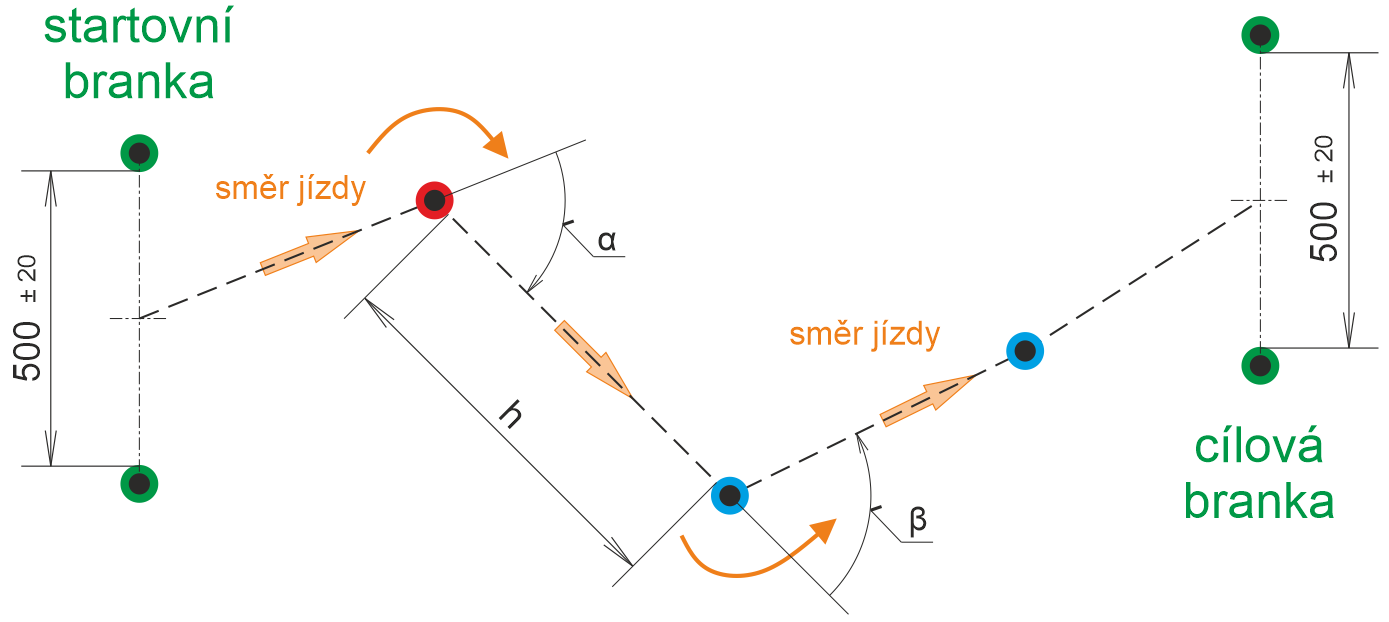
\includegraphics[width=12cm]{vykres_slalom_bezny.png}
	\caption{Schéma dráhy obřího slalomu}
\end{figure}

\newpage

\subsection{Použitý robot}

	Pro řešení úlohy byl použit TutleBot 2. Jeho základnu tvoří zařízení Kobuki, které poskytuje základní funkční prvky: systém pro pohyb robotu, bumper, odometrii. Robot je ovládán přes NUC PC s frameworkem pro softwarový vývoj robotu ROS (Robot Operating System). Dále je na robotu umístěn jeden ze dvou RGBD senzorů: Orbex Astra, nebo Intel Real Sense. %  (pro roboty s číslem 1, 2), (pro roboty s číslem 3-7
	\\
	\\
	\\
	
\begin{figure}[h]
	\centering
	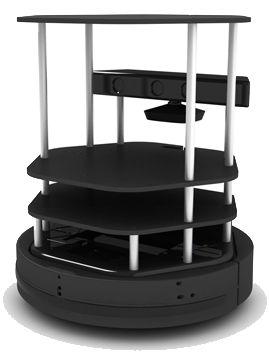
\includegraphics[width=5cm]{turtlebot_2.png}
	\caption{TurtleBot 2}
\end{figure}
	

\clearpage


\section{Návrh řešení a úpravy}

	Původně jsme řešili úlohu druhé úrovně obtížnosti, \uv{Obří slalom}, nakonec jsme ale plynule přešli na úlohu 3 -- \uv{Klasický slalom}, neboť jsme většinu funkcí, které jsou aplikovatelné v obou úlohách, již měli naimplementovanou. Část debuggingu a úprav specifikace byla tedy prováděna při řešení úlohy \uv{Obří slalom}. 

	Z prvu jsme k řešení úlohy přistupovali pomocí co nejjedodušších metod, které jsme později vylepšovali a rozšiřovali, aby byl program robustnější a robot projel trať za co nejnáročnějších podmínek. 
	
	Pro nalezení tyček v obraze jsme stanovili pevné prahy, které jsme nejprve odhadovali z jednoho měření, což se později ukázalo jako nedostačující pro segmentaci obrazu v různých světelných podmínkách. 
	
	Orientace v prostoru měla být původně provedena pouze za pomoci RGB kamery a odometrie. To by ale vedlo ke složitějším výpočtům a pravděpodobně také k chybám a nepřesnostem v jízdě. Začali jsme tedy uvažovat data z hloubkové kamery. 
	
	Pohyb na dráze původně obsahoval projetí středem spojnice dvou po sobě následujících tyček, pokud mají různou barvu. Tento bod jsme později nahradili bodem $x_{0}$ popsaným v podkapitole \uv{Objíždění branky}. 

	
	%Nejprve jsme zkusili následující postup: 	
	
	%\vspace{0.5cm}
	
	%Vektor třetí dimenze jsme si uložili jako {\bf z} a v matici jej nahradili vektorem jedniček -- tím jse převedli matici do homogenních souřadnic. Novou matici jsme označili jako {\bf $M1_{CAM}$}. Následně jsme využili rovnici:

%\begin{equation}
%	{\bf X} = \lambda \cdot {\bf K^{-1}} \cdot {\bf M1_{CAM}},
%\end{equation}
%	kde ${\bf K^{-1}}$ je matice hloubkové kamery se souřadnicemi se středem v kameře získaná funkcí {\it get\_depth\_K()} a $\lambda$ je empiricky zjistěná hodnota. Pro její získání jsme provedli osm měření vzdáleností tyček od sebe s hodnotou $\lambda = 1$. Poté jsme na výsledky aplikovali metodu nejmenších čtverců a dostali hodnotu $\lambda = 429$. 
	
%	Z matice {\bf X} jsme opět odstranili vektor třetí dimenze a nahradili jej vektorem {\bf z}. Výsledná matice {\bf  $M_{CAM}$} byla matice souřadnic se středem v robotu. 
	
%	\vspace{0.5cm}
	
%	Tento postup se ukázal jako nepřesný, robot všechny branky projížděl mírně vlevo. Přestože je neshodil, rozhodli jsme se vynechat použití matice {\it K} po tom, co jsme otestovali, že bez tohoto výpočtu projíždí robot branku přesněji. Chyby byly pravděpodobně způsobeny nepřesným měřením vzdáleností a tedy nepřesnou konstantou $\lambda$.
	
\newpage

\section{Řešení}

\subsection{Segmentace}
	
	Pro nalezení jednotlivých tyček v obraze získaném z RGB kamery jsme zvolili segmentační metodu prahování. Nejprve jsme získali obraz z kamery pomocí funkce {\it get\_rgb\_image()}. Převedli jsme obraz z RGB do HSV barevné reprezentace a zvolili optimální prahové hodnoty. Pro každou barvu jsme experimentálně nalezli práh tak, že jsme RGB kamerou pořídili několik snímků každé tyčky při různém osvětlení. 

\vspace{0.5cm}

\begin{table}[h]
\centering
\begin{tabular}{|p{15mm}|p{15mm}|p{15mm}|p{15mm}|p{15mm}|}
\hline
\bf{Barva} & \bf{$H_{exp}$} & \bf{$H_{diff}$} & \bf{$S_{min}$} & \bf{$V_{min}$}\\
\hhline{|=|=|=|=|=|}
\bf{Zelená} & 65 & 25 & 80 & 40 \\
\hline
\bf{Modrá} & 100 & 25 & 150 & 40 \\
\hline
\bf{Červená} & 2 & 8 & 150 & 40 \\
\hline

% H: stredni hodnota hue, ocekavana
% S: min
% V: min

\end{tabular}

\caption{Tabulka zvolených prahových hodnot, kde: $H_{exp}$ je střední hodnota odstínu, $H_{diff}$ je maximální povolený rozdíl měřené a střední hodnoty odstínu, $S_{min}$ je minimální saturace a $V_{min}$ minimální jas.}

\end{table}

\vspace{0.7cm}

	Dále jsme v obraze detekovali spojité oblasti jako kandidáty pro tyčky pomocí OpenCV funkce {\it connectedComponentsWithStats()}. Odstranění nežádoucích oblastí jsme realizovali pomocí výstupů této funkce -- definovali jsme minimální požadovanou plochu {\it S} a také podmínky pro poměr výšky {\it h} a šířky {\it w}:
	
\begin{equation}
	S > 3000 \; [px],
\end{equation}
 	v případě startovní branky a 

\begin{equation}
	S > 800 [px],
\end{equation}
jinde,

\begin{equation}
	r = \frac{h}{w} = 5.1,
\end{equation}

\begin{equation}
	r_{diff} < 3,
\end{equation}
	kde $r_{diff}$ je rozdíl poměru měřených hodnot a definovaného poměru {\it r}. 

\subsection{Orientace v prostoru}

	Pro orientaci v prostoru jsme využili point cloud. Point cloud je sada bodů, které reprezentují daný objekt v prostoru. Každý bod je charakterizován souřadnicemi {\it x, y, z}. Point cloud získáváme z funkce {\it get\_point\_cloud()} jako matici o velikosti 480 x 640 x 3. 
	
	Při řešení úlohy \uv{Obří slalom} jsme zjistili, že robot vždy projížděl brankou vpravo od jejího středu. Tento posun byl dál umístěním hloubkové kamery, které nebylo přesně ve středu robotu. V implementaci jsme tedy použili posun o tuto konstantu, 3 cm.
	
	 Souřadnice tyčky jsme pak získali podle výsledků segmentace -- vybrali jsme souřadnice všech bodů, které přísluší dané tyčce a spočítali jsme medián v každé souřadnici. Tyto souřadnice poté transformujeme do souřadné soustavy vztažené ke startovní pozici robotu. 
	
	Dále jsme pro orientaci využívali funkcí {\it reset\_odometry()} a {\it get\_odometry()}. {\it Reset\_odometry()} nastaví počátek souřadnic na aktuální pozici robotu, což se provede ihned po spuštění robotu. {\it Get\_odometry()} vrací relativní vzdálenost uraženou od posledního volání {\it reset\_odometry()}. 

\subsection{Pohyb na dráze}

\subsubsection{Hledání startovní branky}
	
	Po spuštění robotu se aktivuje hledání zelené branky. Robot se otáčí, dokud nedetekuje dvě zelené tyčky. Poté změří jejich relativní pozici vůči němu a najede na osu této branky do vzdálenosti půl robotu + 5 cm před ní. Brankou projíždí a zastaví se až v momentě, kdy projede polovina těla robotu. 
	
\subsubsection{Hledání nejbližší tyčky}
	
	Následně robot hledá nejbližší tyčku. Tato úloha se rozděluje na 2 případy:

\begin{itemize}
	
	\item Robot hledá první branku po projetí startem: Otočí se o úhel 30° na obě strany. 
	
	\item Robot hledá branku ve zbytku trati: Otočí se o 60° doprava v případě, že poslední branka, kterou projel, byla červená, nebo se otočí o 60° doleva, pokud poslední branka, kterou projel, byla modrá. 
	

\end{itemize}
	
	Určení nejbližší z tyček pak probíhá pomocí její první a druhé souřadnice (vertikální souřadnici neuvažujeme) -- počítá se eukleidovská vzdálenost robotu od tyčky.  Robot si zapamatuje její barvu i souřadnice. Pokud jde o zelenou tyčku, spustí se stejný proces jako při projíždění startovní brankou. Pokud ne, spustí se objíždění branky. 

\subsubsection{Objíždění branky}

	Robot objíždí branku podle obrázku číslo 3. Pomocí souřadnic detekované tyčky se vypočítají body $x_{0}$, $x_{1}$ a $x_{2}$. Ozn. $o_{1}$ a $o_{2}$ jako spojnice aktuální detekované a předchozí tyčky. Pro velikosti vektorů \textbf{a} a \textbf{b} platí:
	
\begin{equation}	
	 a = r + t + 3,
\end{equation}
\begin{equation}
	b = r + t + 5,
\end{equation}

kde {\it r} je poloměr robotu, {\it t} je poloměr tyčky a konstantay 3, 5 [cm] jsou zvolené rezervy.

	Vektory \textbf{a} a \textbf{b} jsou ortogonální, vektor \textbf{b} je kolmý na osu, a oba vektory se přepočítají po projetí branky, tj. v bodě $x_{2}$.

	Po detekci nové tyčky se vypočítá se nová osa, $o_{2}$, a bod $x_{0}$ je pak ve vzdálenosti $\vert$\textbf{a}$\vert$ od tyčky, u které se robot nachází, ve směru vektoru \textbf{a} a ve vzdálenosti $\vert$\textbf{b}$\vert$ této tyčky ve směru vektoru \textbf{b}, pokud je její barva modrá, nebo ve směru vektoru \textbf{-b}, pokud je její barva červená.

\begin{figure}[h]
	\centering
	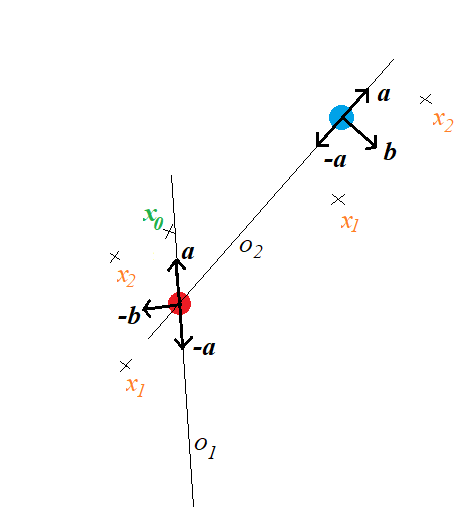
\includegraphics[width=7cm]{schema.png}
	\caption{Schéma objíždění branky}
\end{figure}
	
	Bod $x_{1}$ je vzdálenosti  $\vert$\textbf{a}$\vert$ od detekované tyčky ve směru vektoru \textbf{-a} a vzdálenosti  $\vert$\textbf{b}$\vert$ ve směru vektoru \textbf{b}, pokud její barva je modrá, nebo ve směru vektoru \textbf{-b}, pokud je její barva červená. 

	Bod $x_{2}$ je ve vzdálenosti $\vert$\textbf{a}$\vert$ od detekované tyčky ve směru vektoru \textbf{a} a vzdálenosti $\vert$\textbf{b}$\vert$ ve směru vektoru \textbf{b}, pokud její barva je modrá, nebo ve směru vektoru \textbf{-b}, pokud je její barva červená. 

	Robot projíždí branku postupně po bodech $x_{0}$, $x_{1}$, $x_{2}$. Poté se přepočítá osa a robot pokračuje novými body $x_{0}$, $x_{1}$, $x_{2}$. Pokud následující branka má stejnou barvu jako branka předchozí, robot vynechá bod $x_{1}$. V případě projíždění první branky po startovní brance, robot vynechá bod $x_{0}$.
	
	Po ukončení objíždění branky se vždy znovu aktivuje hledání nejbližší tyčky. 
	
\subsection{Poznámky k implementaci}

\subsubsection{Členění kódu}

	Kód je strukturován do několika hlavních souborů, které jsou v této sekci stručně popsány.
	
	Soubor \emph{main.py} obsahuje hlavní smyčku programu, ve které se pravidelně volá metoda \emph{Driver.drive()}, pomocí které je řidiči umožněno robot ovládat. (Třída \emph{Driver} je diskutována níže.) Dále je zde implementována inicializace hardwaru i softwaru.
	
	Soubor \emph{turtle.py} obsahuje třídu \emph{Turtle}, ve které jsou implementovány wrappery na funkce robotu. Pomocí těchto funkcí může řidič jednoduše získávat data ze senzorů robotu a ovládat jej.
	
	Soubor \emph{driver.py} obsahuje veškerou logiku řízení robotu. Je zde třída \emph{Driver}, která ovládá robot pomocí tzv. \emph{aktivit}. Aktivity -- třídy rozšiřující abstraktní třídu \emph{Activity} -- popisují jednotlivé akce, které robot vykonává, a mohou se skládat z dalších aktivit. (Příkladem takové aktivity může být například aktivita \uv{jet na souřadnice}, která se skládá z dalších pod-aktivit \uv{otočit se} a \uv{jet dopředu}.) Díky tomuto objektovému přístupu je kód přehlednější, modulární a k aktivitám můžeme přistupovat jako k funkcím se vstupními a výstupními hodnotami, přestože jsou to často komplexní akce, jejichž vykonání trvá mnoho cyklů hlavního programu.
	
	V souboru \emph{camera.py} jsou implementovány statické funkce pro zpracování obrazu a dat ze senzorů.
	
	Soubor \emph{CONST.py} obsahuje konstanty úlohy, vlastností robotu, naměřené a empiricky zjištěné konstanty pro segmentaci obrazu i konstanty hlavního programu. Konstanty týkající se logiky ovládání robotu jsou v souboru \emph{driver.py}.
	
\subsubsection{Spuštění programu}

	Pro spuštění programu spustíme soubor \emph{main.py} (Například přikazem \emph{python3 main.py}.) a poté stiskneme tlačítko \uv{B0} na základně robotu. 

\subsubsection{Dodatečné poznámky}

	Během implementace a testování jsme narazili na nečekané chování robotu v případě, že je příliš často volána metoda \emph{Turtlebot.cmd\_velocity(linear, angular)}. Robot se při častém volání této metody choval nekonzistentně a nepohyboval se plynule.

	Proto je v našem kódu nastavování rychlosti robotu rozděleno do dvou metod: \emph{Turtle.keep\_speed()}, která interně volá nativní metodu \emph{Turtlebot.cmd\_velocity(linear, angular)} beze změny rychlosti, a \emph{Turtle.set\_speed(linear, angular)}, která přenastaví hodnoty rychlosti robotu uvnitř třídy \emph{Turtle} bez volání nativní metody \emph{Turtle.set\_speed(linear, angular)}. Využití těchto dvou metod je na programátorovi řidiče, doporučujeme ale volat metodu \emph{Turtle.keep\_speed()} pouze jednou v každém volání \emph{Driver.drive()}, a ve zbylé logice řidiče a aktivit používat pouze metodu \emph{Turtle.set\_speed(linear, angular)}.

\newpage

\section{Závěr}
 	
 	Funkčnost našeho řešení jsme ověřili na několika drahách, otestovali jsme projíždění v limitních -- jak světelných, tak vzdálenostních -- podmínkách. Naše řešení je robustní vůči světelným podmínkám. Hlavním nedostatkem implementace je chybějící transformace souřadnic mezi RGB a hloubkovou kamerou. Pokud nastane situace, že se tyčky překrývají v zorném poli robotu, může robot změřit souřadnice jedné tyčky a barvu druhé. 
 	
 	Naše implementace by se dala rozšířit o automatický výpočet jasu obrazu z RGB kamery, pomocí čehož by se automaticky přepočítaly používané konstanty barev. Dále by se daly přepočítat souřadnice získané z RGB a hloubkové kamery pomocí funkce {\it get\_depth\_K()} a rovnice:

\begin{equation}
	{\bf X} = \lambda \cdot {\bf K^{-1}} \cdot {\bf M_{CAM}}.
\end{equation}
 	
 	

\subsection{Návrh modifikace úlohy, poznámky}

\subsubsection{Porovnání úloh 2 a 3}

	Vzhledem k tomu, že jsme si vyzkoušeli splnit jak úlohu 2 \uv{Obří slalom}, tak úlohu 3 \uv{Klasický slalom}, máme možnost úlohy dobře porovnat. K řešení úlohy 3, která by měla být \uv{obtížnější}, jsme využili -- po drobných úpravách -- většinu funkcí, které jsme napsali pro úlohu 2. Přibylo především vymyšlení logiky objíždění tyčky. Naopak jsme se nemuseli věnovat hledání druhé tyčky branky do páru, které bylo navíc v limitních případech problematické, protože druhá tyčka branky nemusela být v zorném poli kamery. Po celkovém shrnutí je podle našeho názoru úloha 3 mírně jednodušší než úloha 2. 
	
\subsubsection{Nedostatek tyček v laboratoři}

	V laboratoři jsme měli k dispozici velký počet robotů, ale malý počet tyček. Vzhledem k tomu, že v laboratoři chtělo často testovat více týmů než dva najednou, stávalo se, že tyčky na další týmy nevyzbyly. Abychom mohli ladit náš program i v době, kdy bylo v laboratoři více týmů, vyrobili jsme si tyčky svoje (se stejnými rozměry jako poskytnuté). 

\subsubsection{Návrh na modifikaci}
	
	Jako modifikaci úlohy pro příští rok navrhujeme například úkol posouvat robotem barevné krabice na značky odpovídající barvou dané krabici. 
	


\end{document}